\chapter{Public Key Infrastructure - PKI}

\section{Public Key Distribution Paradigms}

\begin{flushleft}

    Il problema alla base della crittografia simmetrica è la distribuzione della chiave segreta simmetrica, che può essere risolto dalla crittografia asimmetrica. Cosa comporta: 
    \begin{itemize}[nosep]
        \item come distribuiamo in modo \textbf{autentico} le chiavi pubbliche?
        \item di chi o di cosa ci fidiamo per la distribuzione delle chiavi pubbliche?
        \item chi è il nostro punto di fiducia (\textit{trust anchor})?
    \end{itemize}

    Abbiamo la necessità di \textbf{autenticare la chiave pubblica}. È una \textit{challenge} che riguarda l'intero sistema: \textbf{requisiti}, \textbf{vincoli}, \textbf{scalabilità}, \textbf{usabilità}, \textbf{\textit{trust policies}}, ecc.

    \smallskip

    Metodi per autenticare la chiave pubblica:
    \begin{enumerate}[nosep]
        \item \textbf{\textit{Trust-on-first-use (TOFU)}}: la prima volta che scambiamo chiavi, assumiamo che non si venga attivamente attaccati - ad esempio \textbf{SSH}.
        \item \textbf{\textit{Out-of-band verification}}: viene utilizzato un canale sicuro per l'invio della chiave pubblica o un suo rappresentante - ad esempio chiamate di persona, mezzi in generale più costosi \\ 
        $\Rightarrow$ qualcosa che ci permette di validare \textbf{AuthN}.
        \item \textbf{\textit{Delegated approaches $\rightarrow$ Trust third parties}}: lasciamo che un'altra entità autentichino le chiavi pubbliche - qualcuno di cui ci fidiamo firma la chiave pubblica per valutarne l'autenticità. \\
        $\Rightarrow$ riduciamo il tutto ad un problema di \textbf{\textit{trust management}}.
    \end{enumerate}

    \newpage

    \textcolor{red}{\textbf{\textit{Trusted third party [ abstract ]}}} \\
    Alice e Bob vogliono comunicare, hanno un ``amico'' in comune Carl di cui entrambi si fidano. Durante il \textit{key exchange} bob invia la sua \textit{public key} e anche la $pk_b, \sigma_{carl}$ dove $\sigma_{carl} = \text{sign}(sk_c, pk_b)$

    \begin{figure}[h]
        \centering
        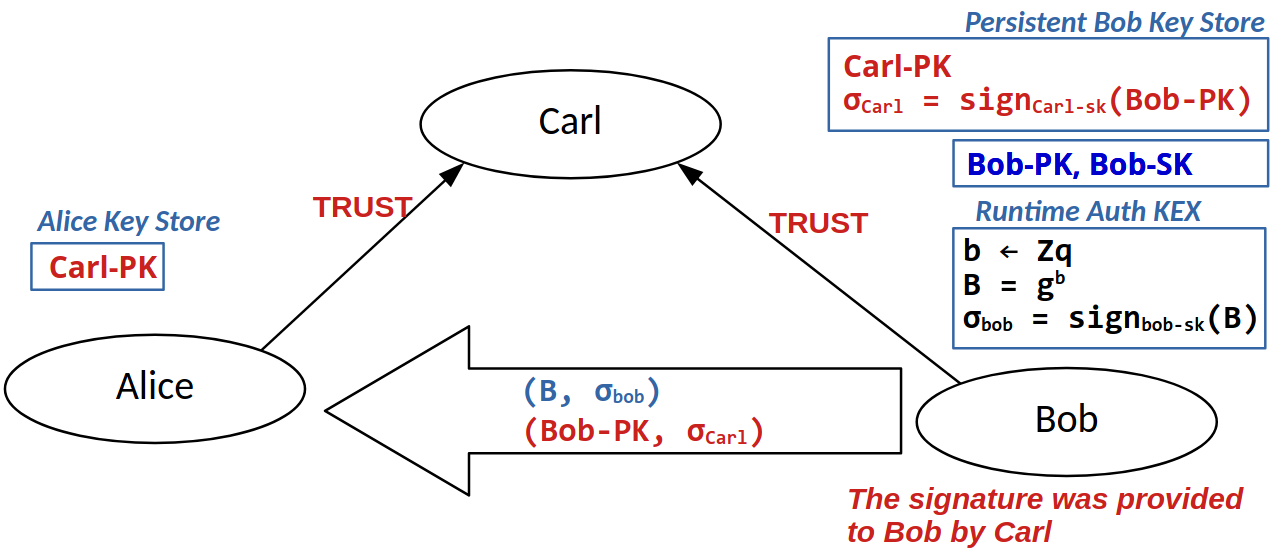
\includegraphics[width=0.75\textwidth]{img/ab_ca.png}
    \end{figure}

    Il paradigma di \textit{trusted third part} può essere diviso in due macro-aree:
    \begin{itemize}[nosep]
        \item \textbf{\textit{Centralized}}: una o poche entità dedicate fungono come \textit{trusted third parties} - ad esempio \textbf{\textit{Public Key Infrastructure}} come la \textbf{\textit{Certification Authority}}.
        \item \textbf{\textit{Distributed}}: molte entità non dedicate si comportano come \textit{trusted third parties}. In generale, le stesse entità che agiscono all'interno del protocollo fungono anche da intermediari per valutare l'identità di altre entità - ad esempio \textbf{\textit{OpenPGP Web of Trust}}.
    \end{itemize}

    Distribuire chiavi pubbliche non è sufficiente, è infatti necessario associare il materiale crittografico a \textbf{metadati} che possono essere: \textcolor{red}{\textbf{[1] ``tecnici''}} come ad esempio i nomi degli algoritmi, periodo di validità (informazioni di revoca), altre informazioni dipendendi anche dai protocolli utilizzati - come ad esempio le \textbf{\textit{Certification Transparency - CT}} e i \textbf{\textit{SignedCertificateTimestamps - SCTs}}. \textcolor{red}{\textbf{[2] \textit{Claims}}} che comprendono informazioni su come può essere utilizzata l'attestazione come ad esempio: l'ambito (regole di autorizzazione), \textit{audience} (per chi è stata rilasciata l'attestazione), informazioni sull'autorizzazione (quali servizi e risorse) e metadati di livello superiore (informazioni sull'identità, informazioni legali, ecc).

    \medskip

    \textcolor{red}{\textbf{\textit{Cryptography Attestations}}}: è una struttura dati autenticata crittograficamente che lega materiale crittografico ai metadati. Il nome più famoso è quello di \textbf{\textit{Web Certification (x509)}} che sono le \textit{cryptography attestations} scambiate a livello transporto (\textbf{TLS}). Due esempi sono:
    \begin{enumerate}[nosep]
        \item \textbf{\textit{JOSE}} (\textit{javascript objects signing and encryption framework}): è lo standard per cifrare e firmare informazioni con i \textbf{\textit{JSON Web Token - JWT}}, comprende dei sottostandard come \textbf{\textit{JWE - Encryption}}, \textbf{\textit{JWS - Signature}} e \textbf{\textit{JWK - Key Storage}}.
        \item \textbf{\textit{COSE}} (\textit{cbor object signing and encryption framework}): può essere considerata la versione \textbf{binaria} di \textbf{JOSE} è normalmente utilizzata per l'ottimizzazione dello spazio - utilizzata in protocolli come: COAP, FIDO2-CTAP2.
    \end{enumerate}
    Sono due set di standard per l'autenticazione e/o la crittografia di strutture dati, che esulano dal contesto in cui vengono applicati.

    \medskip

    \textcolor{red}{\textbf{\textit{Web Certificate $\rightarrow$ x509 Standard}}}: permette di specificare i campi per i \textbf{metadati} e quelli per gli \textbf{schemi crittografici}, queste informazioni sono descritte tramite un \textit{formal interface description language - IDL} chiamata \textbf{\textit{Abstract Syntax Notation One - ASN.1}}

    \begin{figure}[h]
        \centering
        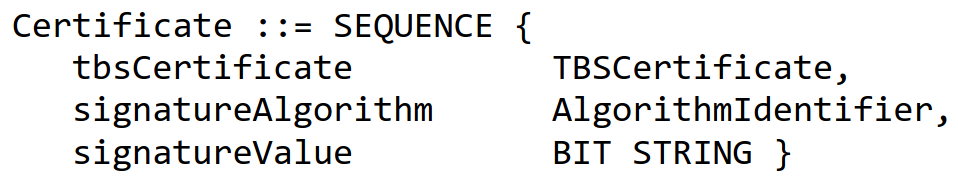
\includegraphics[width=0.75\textwidth]{img/x509.png}
        \caption{Esempio di un x509v3 descritta formalmente con ASN.1}
    \end{figure}

    Questa \textit{abstract view} del certificato non viene mai inviata/memorizzata \textit{as is}, ma viene utilizzato uno schema di \textbf{\textit{encoding}}. Per evitare problemi di sicurezza dovuti alla canonizzazione delle informazioni, abbiamo bisogno di un \textbf{\textit{encoding scheme}} che produce una rappresentazione \textbf{unica} delle informazioni del certificato.
    \begin{itemize}[nosep]
        \item \textbf{\textit{DER - Distinguished Encoding Rules}}: che è uno schema \textbf{deterministico} di codifica binaria.
        \item \textbf{\textit{PEM - Privacy Enhanced Mail}}: il nome ricorda l'uso originario del metodo di \textit{encoding}, ma oggigiorno è utilizzato per molti contesti. Il \textbf{PEM} non è altro un \textbf{base64} con l'aggiunta di \textbf{\textit{tags}} che permettono di essere gestiti più semplicemente dagli utenti e scambiati attraverso protocolli testuali.
    \end{itemize}

    Lo standard \textbf{PEM} non viene unicamente utilizzato per memorizzare certificati x509, ma ance informazioni su materiale crittografico, ogni blocco è definito da un tag iniziale e uno finale
    
    {\centering
        \texttt{----- BEGIN <block-type> -----}  \\
        \textbf{\texttt{<data>}} \\
         \texttt{----- END <block-type> ------}.
    \par}
    
    I dati presenti all'interno dei tags sono \textit{encodati} \textbf{base64} e possono essere in chiaro o cifrati. \textbf{DER} può includere differenti tipologie di dati, ma queste informazioni non sono facilmente riconoscibili dall'utente e il \textit{parsing} da parte di un applicativo è obbligatorio. 

    \medskip

    Un file \textbf{PEM} può avere l'estensione \texttt{.pem}, ma è possibile trovare altre estensioni dipendentemente dal contesto:
    \begin{itemize}[nosep]
        \item \textbf{\texttt{.key}}: vengono memorizzate le chiavi private.
        \item \textbf{\texttt{.pub}}: vengono memorizzate le chiavi pubbliche.
        \item \textbf{\texttt{.crt}}: memorizzato i \textit{web certificates}.
        \item \textbf{\texttt{.csr}}: memorizzano \textbf{\textit{Certificate sign request CSR}}.
        \item \textbf{\texttt{.crl}}: memorizzano \textbf{\textit{Certification revocation list CRL}}
        \item altri..
    \end{itemize}

    Gli standard x509 e DER/PEM sono i più comuni sul web, ma ne esistono altri con lo stesso obiettivo, ad esempio \textbf{[1] \textit{PKCS\#7 Cryptography message syntax}} o \textbf{[2] \textit{PKCS\#12 PFX}} è \textit{microsoft-friendly}. \\
    I certificati x509 e DER/PEM sono complessi e tipicamente vengono utilizzati solo per i \textit{web certificates} attraverso strumenti standard (openssl, cfssl); non sono flessibili e non è conveniente l'utilizzo in altri impostazioni.

\end{flushleft}

\newpage

\section{Public Key Infrastructure Architecture}

\begin{flushleft}

    La \textbf{PKI} è un approccio centralizzato e delegato per la distribuzione delle chiavi pubbliche. Le \textbf{terze parti fidate} sono chiamate \textbf{\textit{Certification Authorities}}, una \textbf{CA} rilascia un certificato che \textit{binda} una \textit{public key} ad un'\textit{entity} (persona, ruolo, organizzazione e dispositivi). Ogni entità può includere \textit{identification information} (nome, la nazione, lo stato e la città) ma possono includere anche altre informazioni o metadati.

    \smallskip

    \begin{figure}[h]
        \centering
        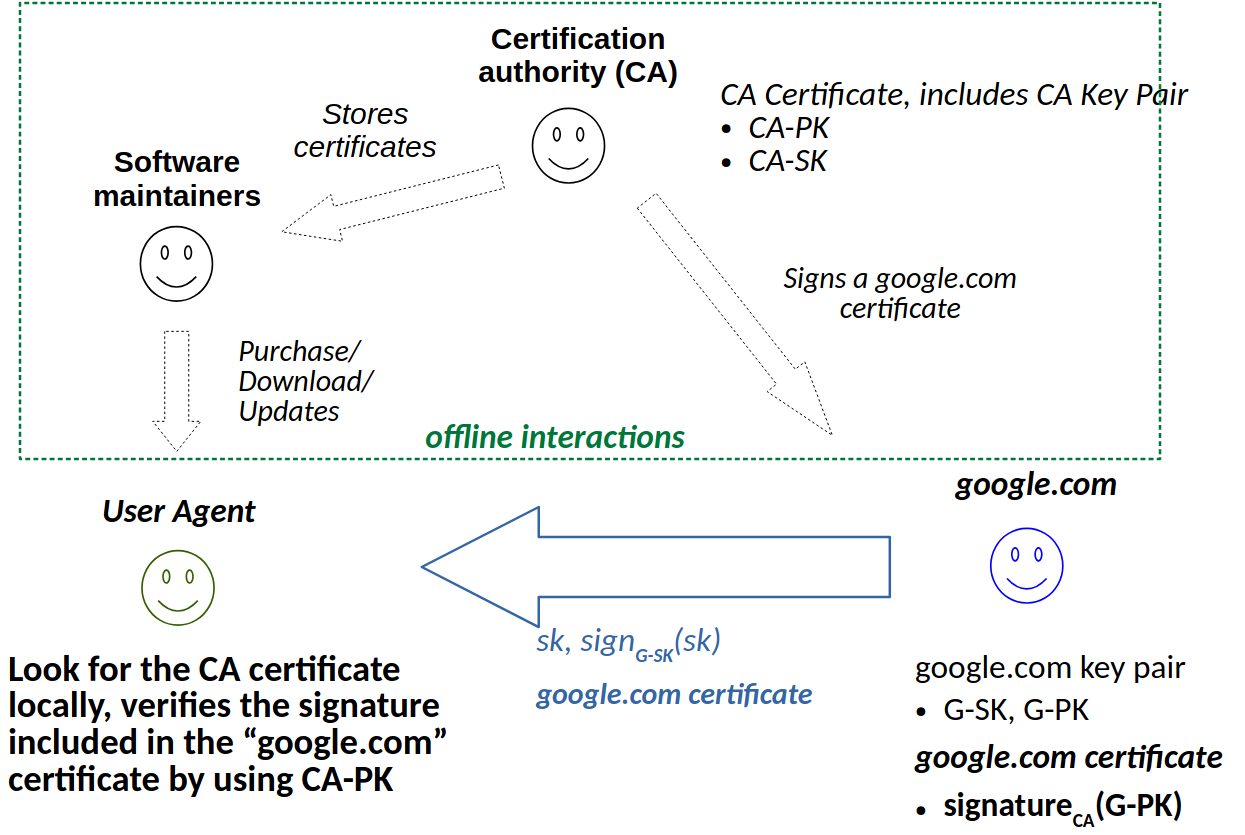
\includegraphics[width=\textwidth]{img/ca_mf.png}
    \end{figure}

    \newpage

    \textcolor{red}{\textbf{\textit{Certificate Chain}}} \\
    Un server ha un certificato emesso da un \textbf{\textit{intermediate CA}}, che a sua volta ha un certificato emesso da un'altra \textit{intermediate CA} oppure \textbf{\textit{root CA}} (pre-installate negli \textit{OS} e nei \textit{browser web} per quanto riguarda le politiche di \textit{governance}) - l'autorizzazione di nuove \textit{root CA} o la revoca di quelle esistenti è un argomento di discussione aperta all'interno della \textit{security communities}.

    \smallskip

    Per la verifica \textit{end-user} dei certificati, il client deve verificare tutta la \textbf{catena di certificati} fino a ché non trova un \textbf{certificato fidato}. Un server può inviare l'intera catena dei certificati o assumere che il client conosca molti ``famosi'' \textit{intermediate CA} e invi unicamente il proprio certificato. \\
    La valida del certificato richiede di \textbf{verificare la \textit{signature}} dell'emittente e \textbf{verificare i metadati in maniera coerente con l'applicazione}, per poi passare a tutta la catena e verificare che il certificato non sia presente nella \textbf{\textit{CA certificate revocation list}}. Con il comando:
    
    {\centering
        \texttt{openssl s\_client -connect google.it:443}
    \par}

    Per i \textbf{certificati Web}, il \textbf{\textit{Common Name (CN)}} o il \textbf{\textit{Subject Alternative Name (SAN)}} devono corrispondere al nome di dominio completo (\textbf{FQDN}) del sito.
    \begin{itemize}[nosep]
        \item Se provi ad accedere a un sito HTTPS usando un nome host diverso (ad esempio modificando il file hosts), riceverai un errore di certificato.
    \end{itemize}
    
    Per leggere tutti i dettagli di un certificato:

    {\centering
        \texttt{openssl x509 -noout -text -in <certificato>}
    \par}

\end{flushleft}

\section{Web Certification: Release and Revocation}

\begin{flushleft}
    Le \textbf{CA} possono rilasciare certificati web con durata massima di \textbf{un anno}, la durata è specificata all'interna del certificato, che quindi dichiara la propria scadenza ``naturale'', ma è possibile \textbf{revocare} un certificato prima della data di scadenza, ma quest'azione presenta diverse problematiche, per questo motivo in passato i certificati avevano una durata più lunga.

    \smallskip

    Per ottenere un certificato valido da una \textbf{\textit{Certification Authority (CA)}} è necessario generare una richiesta di firma (\textit{Certificate Sign Request, CSR}), preferibilmente su una macchina sicura e offline. Il processo prevede: 
    \begin{enumerate}[nosep]
        \item la \textbf{creazione di una coppia di chiavi}, mantenendo segreta la chiave privata (tipicamente RSA con modulo di almeno 2048 bit);
        \item la generazione della \textbf{CSR};
        \item l'invio della \textbf{CSR} alla CA (solitamente a pagamento);
        \item la memorizzazione sicura della chiave privata sul server Web, con permessi di accesso molto restrittivi (sola lettura per \texttt{root}); idealmente, l'uso di un \textbf{\textit{Hardware Security Module (HSM)}} per la protezione della chiave.
    \end{enumerate}

    \smallskip

    \textcolor{red}{\textbf{Revoca dei Certificati}} \\
    Ogni certificato digitale possiede una ``data di scadenza'' che viene verificata dal client in base al proprio orologio locale. Questa data è parte integrante del certificato firmato digitalmente, quindi \textbf{non può essere modificata} senza invalidare la firma. Tuttavia, può rendersi necessario revocare un certificato prima della sua naturale scadenza, ad esempio in caso di \textbf{compromissione della chiave segreta} del server (come nel caso della vulnerabilità Heartbleed). 

    Le \textbf{\textit{Certification Authority (CA)}} inseriscono all'interno dei certificati x509 le informazioni necessarie alla gestione della revoca, specificando gli endpoint pubblici dove tali informazioni possono essere reperite. I due principali meccanismi di revoca sono:

    \begin{itemize}[nosep]
        \item \textbf{\textit{Certificate Revocation Lists (CRL)}}: liste periodicamente aggiornate pubblicate dalle CA che elencano tutti i certificati revocati prima della scadenza. I client devono consultare queste liste per verificare lo stato dei certificati, ma le \textbf{CRL} possono diventare molto grandi e causare ritardi nella verifica.
        
        \item \textbf{Online Certificate Status Protocol (OCSP)}: protocollo che permette di interrogare in tempo reale la CA per ottenere lo stato (valido/revocato) di un certificato specifico. La richiesta viene inviata via HTTP e la risposta è firmata dalla CA. Per migliorare le prestazioni, si utilizza l'\textbf{OCSP Stapling}, in cui il server Web include nella connessione una risposta OCSP recente e firmata, evitando al client di contattare direttamente la CA.

        \begin{figure}[h]
            \centering
            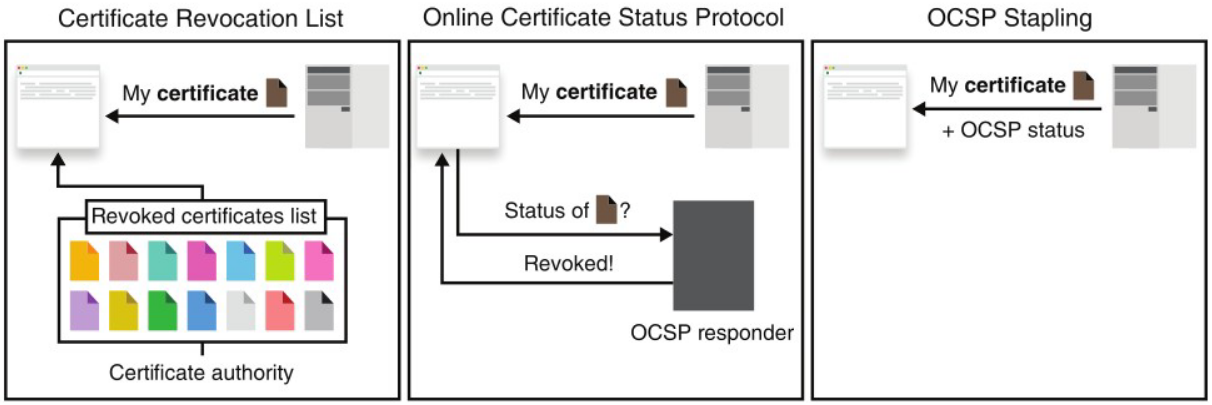
\includegraphics[width=0.75\textwidth]{img/ocsp_sta.png}
        \end{figure}
    \end{itemize}

    La revoca dei certificati presenta diverse problematiche, soprattutto in presenza di \textbf{attacchi attivi}. Un attaccante che riesce a sottrarre un certificato può anche impedire o compromettere i meccanismi di verifica online della revoca al momento dell'accesso. Esempi comuni includono attacchi \textbf{MitM} che restituiscono risposte OCSP o CRL obsolete (\textit{stale attacks}), oppure attacchi di \textit{denial of service} che bloccano l'accesso ai server OCSP o ai punti di distribuzione delle CRL. In questi casi, sorge il dubbio su quale debba essere il comportamento predefinito: considerare il certificato revocato (\textit{implicit revoke}) o valido (\textit{implicit non-revoke}) in assenza di informazioni esplicite di revoca. Attualmente, la scelta adottata dalla maggior parte dei browser è quella di considerare il certificato \textbf{ancora valido} se non si riesce a ottenere informazioni di revoca, ad esempio in ambienti con \textit{captive portal}.

    Per mitigare questi problemi, l'obiettivo è evitare il controllo della revoca in tempo reale. Questo si ottiene aggiornando localmente le liste di certificati revocati (CRL) non appena disponibili. Il processo prevede due fasi:
    \begin{enumerate}[nosep]
        \item \textbf{Monitoraggio delle CRL} pubblicate dalle \textit{Certification Authority}. Per migliorare l'efficienza, vengono selezionate solo revoche rilevanti, ad esempio in base al tipo di certificato (\textbf{\textit{Domain validate - DV}}, \textbf{\textit{Extended Validation}}) o al \textbf{codice di revoca}.
        \item \textbf{Distribuzione delle revoche ai browser}, tramite aggiornamenti software o sistemi di blacklist. 
    \end{enumerate}

\end{flushleft}

\section{Types of Public Certification Authorities}

\begin{flushleft}

    \textbf{Tipologie di Certificati}:
    \begin{itemize}[nosep]
        \item \textbf{\textit{Domain Validation}}: verifica solo che il richiedente abbia il controllo del dominio; è automatico, veloce ed economico ma non garantisce sull'identità dell'organizzazione.
        \item \textbf{\textit{Extended Validation}}: richiede una verifica approfondita dell'identità dell'organizzazione (documenti legali, esistenza reale, ecc); è più costoso e più lento, ma visualizza il nome legale dell'organizzazione nel certificato e quindi nel web.
    \end{itemize}

    Le \textbf{CA} sono \textit{trusted third parties}, il vantaggio del sistema \textbf{PKI} è che è un'architettura \textbf{scalabile} per le comunicazione cifrate e autenticazione sicura all'interno di una rete privata. Per la verifica tramite le \textbf{CA} ci deve essere il \textit{trust} di tutti gli anelli della catena che lo compongono. Lo svantaggio è che bisogna ``fidarsi''. Se si vuole evitare le \textbf{\textit{public CA}} è possibile configurare delle \textbf{CA private} per uso interno - possono essere utilizzate da tutti i \textit{tool} e applicazioni che supportano \textbf{PKI}. I \textbf{\textit{Self-signed certificates}} rappresentano un approccio semplificato per i certificati privati. La \textit{public key} del server viene firmata usando il proprio certificato, andando a ricadere su una distribuzione \textbf{\textit{out-of-bound}} o su \textbf{\textit{TOFU}}.

\end{flushleft}

\newpage

\section{Problemi nelle Trusted Thrid Parties e CT}

\begin{flushleft}
    
    Il problema è stato spostato nell'aggiungere \textbf{CA} \textit{ad-hoc}, infatti un avversario potrebbe compromettere una chiave privata di un server valido oppure le \textbf{CAs} che vengono aggiunte al nostro \textit{device} potrebbero essere ``malevole''. \\
    $ \qquad \Rightarrow$ \textbf{\textit{Hardening public PKI}}

    \smallskip

    È possibile implementare soluzioni \textit{ad-hoc}: \textbf{\textit{restricted trusted CAs}} - \textit{whitelist} o \textit{blacklist} - oppure si potrebbe andare a mettere una ``pezza'' sul protocollo - \textbf{\textit{HTTP pinning}} o una soluzione a livello ``globale'' come \textbf{\textit{Certificate Transparency}}
    \begin{itemize}[nosep]
        \item \textbf{\textit{Whitelisting CAs}}: è la pratica di configurare una lista di \textbf{CA} considerate affidabili per validare certificiati digitali; questa lista può essere gestita a livello di sistema operativo (\textbf{OS}) influenzando così tutte le applicazioni, oppure a livello del singolo \textit{browser} che può avere una sua lista di \textbf{CAs} indipendentemente dal sistema operativo.
        \item \textbf{\textit{HTTP Pinning}}: tecnica di sicurezza che permette a un client di ``fissare'' (\textbf{pin}) un certificato o una chiave pubblica specifica per un sito web, così da accettare solo certificato nelle future connessioni, prevedendo attacchi \textbf{MitM}.
        \item \textbf{\textit{Certificate Transparency}}: meccanismo che prevede la pubblicazione di tutti i certificati emessi da una \textbf{CA} su log pubblici. Questo consente di rilevare rapidamente certificati fraudolenti o emessi senza autorizzazione, migliorando la trasparenza e la sicurezza del sistema di certificazione.
    \end{itemize}

    \begin{figure}[h]
        \centering
        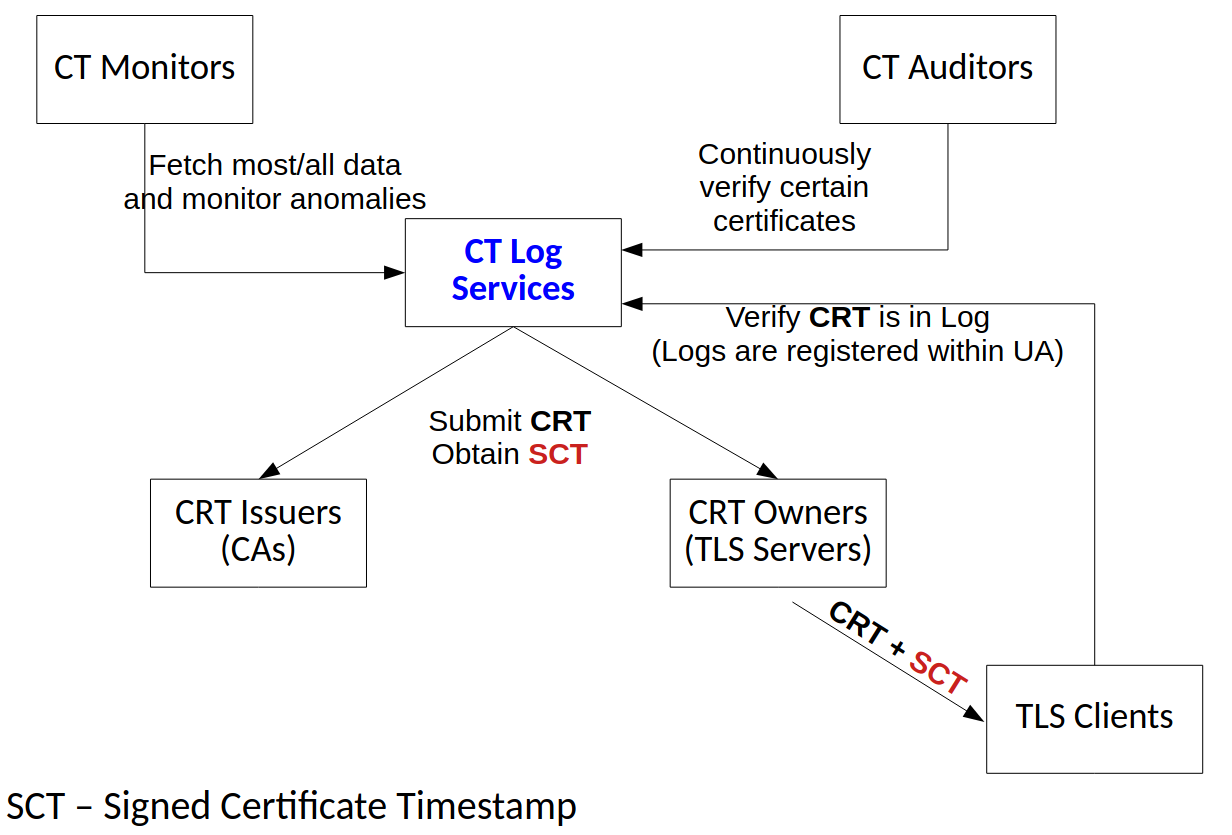
\includegraphics[width=0.75\textwidth]{img/ct_arc.png}
    \end{figure}

    \textbf{\textit{Certificate Transparency}} \\
    Le \textbf{CT} sono un sistema di controllo pubblico e trasparente che permette di monitorare tutti i certificati emessi dalle \textbf{CA} per prevenire emissioni fraudolente o non autorizzate. I ruoli e le azioni principali sono:
    \begin{itemize}[nosep]
        \item \textbf{\textit{Issuer CA}}: è l'ente che emette il certificato (\textbf{CA}), quando un certificato viene emesso, lo inviano a uno o più log pubblici delle \textbf{CT}, questo viene fatto per rendere pubblica l'emissione del certificato in modo da permetterne il controllo esterno.
        \item \textbf{\textit{TLS Server}}: è il titolare del certificato, ovvero l'entità per cui è stato emesso.
        \item \textbf{\textit{CT Log Services}}: ricevono e memorizzano i certificiati in una struttura \textit{append-only} che quindi non è modificabile e neanche cancellabile; i log sono pubblici e implementano una struttura verificabile - ad esempio un \textbf{MHT} - per assicurarsi l'integrità e la non manomissione.
        \item \textbf{\textit{CT Monitors \& Auditors}}: scaricano e analizzano regolarmente i log pubblici per identificare certificati sospetti o non autorizzati permettono di rilevare tempestivamente eventuali certificati fraudolenti o emessi senza consenso.
        \item \textbf{\textit{TLS Client}}: quando viene visitato un sito, verificano il certificato presentato che quello presente nei log CT, controllando tramite \textit{proof} la presenza del certificato nei log - tramite \textbf{SCT - \textit{Signed Certificate Timestamp}} - ottenuto dal certificato stesso o durante l'\textit{handshake TLS} questo permette di garantire che il certificato sia pubblico e tracciabile migliorando la sicurezza e la fiducia.
    \end{itemize}

\end{flushleft}